\section{Results}\label{sec:results}

All results are aggregated across 10 seeds per arm.  Per-seed
trajectories live at \texttt{eval/results/theorem\_6/\{arm\}/seed\_*.json}.
The analysis pipeline
(\texttt{eval/convergence/analysis\_theorem\_6.py}) produces the
machine-readable summary at \texttt{eval/results/theorem\_6/summary.json};
numbers reported here are copied verbatim from that file.  Because
the reflection LM is non-deterministic, the tables in this section
are one sweep; §\ref{sec:results-variance} reports an $N=10$
replication, and where a single-sweep point estimate is not robust
across that replication the replication's range is the result of
record.

\subsection{Convergence rate per arm}

Table~\ref{tab:paper6-convergence-rate} reports the fraction of
runs that reached the predicate $\max \mathbf{x} \le \tau$ on the
validation set within the 50-iteration budget.

\begin{table}[h]
\caption{Convergence rate within 50 iterations (10 seeds per arm,
Wilson 95\% CIs).}
\label{tab:paper6-convergence-rate}
\centering
\small
\begin{tabular}{lccc}
\toprule
Arm & Converged / N & Rate & 95\% CI \\
\midrule
cert-binary       & 10/10 & 1.000 & [0.722, 1.000] \\
scalar            & 10/10 & 1.000 & [0.722, 1.000] \\
scalar-evidence   & 10/10 & 1.000 & [0.722, 1.000] \\
\bottomrule
\end{tabular}
\end{table}

\subsection{Mutations-to-convergence}

Table~\ref{tab:paper6-mutations} reports mean iterations to
convergence per arm; non-converged runs are imputed at the
budget (50).

\begin{table}[h]
\caption{Mean iterations to convergence per arm, with
Mann-Whitney U comparison (\texttt{alternative="less"}) and
rank-biserial effect size (positive = treatment dominates).}
\label{tab:paper6-mutations}
\centering
\small
\begin{tabular}{lcccc}
\toprule
Arm & Mean iters & U & $p$ & Effect size \\
\midrule
cert-binary (treatment)   & 1.0 & ---  & ---   & ---  \\
scalar                    & 2.0 & 35.0 & 0.039 & 0.30 \\
scalar-evidence           & 1.0 & 50.0 & 1.000 & 0.00 \\
\bottomrule
\end{tabular}
\end{table}

\subsection{Convergence CDF}

Figure~\ref{fig:paper6-cdf} shows the empirical cumulative
distribution function of mutations-to-convergence across arms.  At
iteration $k$, each arm's curve gives the probability that a run
had converged by iteration $k$ or earlier.

\begin{figure}[h]
\centering
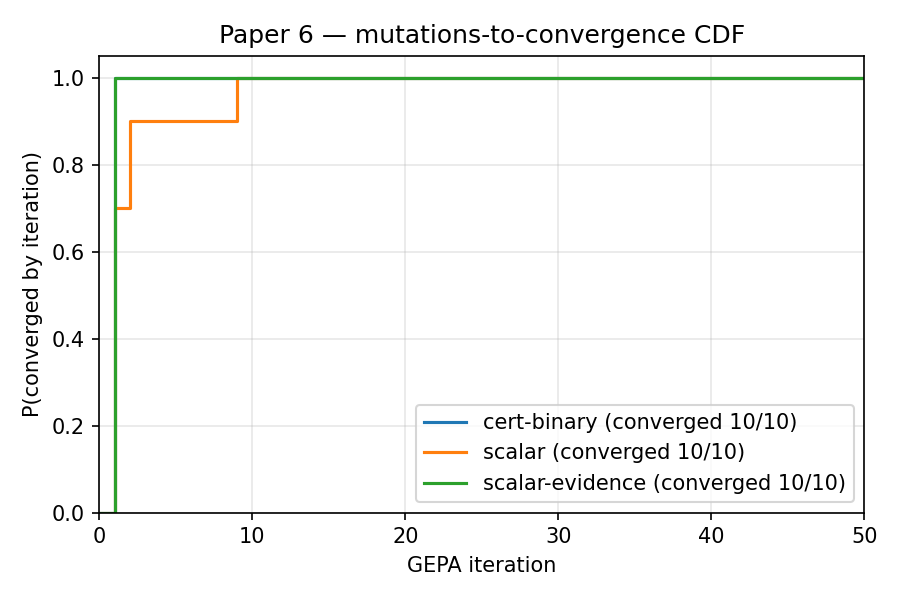
\includegraphics[width=0.8\linewidth]{../../eval/results/theorem_6/cdf.png}
\caption{Empirical CDF of iterations to convergence.  Lines that
reach 1.0 faster indicate arms that converge more reliably.}
\label{fig:paper6-cdf}
\end{figure}

\subsection{Ablation: minimal vs default obligation formatter}

On seeds 0--4, we compare cert-binary run with
\texttt{default\_obligation\_formatter} against cert-binary run with
a minimal formatter (\texttt{"constraint violated: window k"}, no
numbers, no theorem framing).  Table~\ref{tab:paper6-ablation}
reports mean iterations for each.

\begin{table}[h]
\caption{Formatter ablation on seeds 0--4 (cert-binary only).}
\label{tab:paper6-ablation}
\centering
\small
\begin{tabular}{lc}
\toprule
Formatter & Mean iters \\
\midrule
default (numbers + theorem framing) & 1.0 \\
minimal (window index only)         & 1.0 \\
\bottomrule
\end{tabular}
\end{table}

\subsection{Run-to-run replication}\label{sec:results-variance}

The reflection LM is non-deterministic, so the tables above are a
single sweep.  We re-ran the full protocol $N=10$ times
(\texttt{eval/convergence/theorem\_6\_variance.py}; aggregate at
\texttt{eval/results/theorem\_6/variance\_summary.json}), holding
GEPA's seed and the data seeding fixed so the only varying factor is
LM sampling.  Per-arm mean iterations, reported as
median~[min,~max] over the 10 repetitions:

\begin{table}[h]
\caption{Run-to-run replication ($N=10$): per-arm mean iterations
and the cert-binary~vs~scalar-evidence comparison.}
\label{tab:paper6-variance}
\centering
\small
\begin{tabular}{lcc}
\toprule
Arm & Mean iters: median [min, max] & \\
\midrule
cert-binary       & 1.0 [1.0, 1.0] & zero variance \\
scalar-evidence   & 1.0 [1.0, 1.1] & near-zero variance \\
scalar            & 1.7 [1.2, 6.5] & high variance \\
\bottomrule
\end{tabular}
\end{table}

Cert-binary and scalar-evidence are Mann-Whitney-indistinguishable
in $10/10$ repetitions ($p$ range $[0.18,~1.00]$, cert-binary never
slower), and the $\le 0.75$ gate is cleared in $0/10$ --- so the Null
verdict does not depend on the single sweep.  The exact $p=1.000$ and
the scalar mean of $2.0$ in Tables~\ref{tab:paper6-mutations} are
single draws, not robust values.  The replication's sharpest signal
is the variance itself: see §\ref{sec:variance} for the
variance-reduction reading.

\subsection{Honest verdict}

\textbf{Null} per the predeclared gate.  The ratio
$\bar n_{\text{cert-binary}}\,/\min(\bar n_{\text{scalar}}, \bar
n_{\text{scalar-evidence}}) = 1.0\,/\min(2.0, 1.0) = 1.00$ does not
clear the $\le 0.75$ threshold, and the $p$-value against the
stronger baseline (\textit{scalar-evidence}) is $1.000$ in the
reported sweep (indistinguishable in all $10/10$ replications;
§\ref{sec:results-variance}).  Theorem~3
remains a conjecture rather than an accepted theorem for this task.
The ablation in §\ref{sec:ablation} informs which pipeline stage
carries what signal; see also the discussion (§\ref{sec:discussion})
for the cert-binary~vs~scalar-evidence parity and the
cert-binary~vs~scalar gap.
